\documentclass[11pt,a4paper]{article}

\usepackage{fontspec}
\usepackage[bidi=default]{babel}
\babelprovide[import,main]{spanish}
\usepackage[margin=2.5cm]{geometry}
\usepackage{amsmath,amssymb}
\usepackage{booktabs,tabularx,array}
\usepackage{graphicx}
\usepackage{xcolor}
\usepackage{listings}
\usepackage{caption}
\usepackage{float}
\usepackage{tikz}
\usepackage{pgfplots}
\usepackage{setspace}
\usepackage{fancyhdr}
\usepackage[colorlinks=true,linkcolor=blue!50!black,urlcolor=blue!50!black,citecolor=blue!50!black]{hyperref}
\usetikzlibrary{positioning,shapes.geometric,arrows.meta,calc,fit,backgrounds}
\pgfplotsset{compat=1.16}

\AtBeginDocument{\renewcommand{\tablename}{Tabla}\renewcommand{\listtablename}{Índice de tablas}\renewcommand{\lstlistingname}{Código}}
\sloppy
\emergencystretch=3em
\setstretch{1.08}
\captionsetup{font=small,labelfont=bf}
\pagestyle{fancy}
\fancyhf{}
\fancyhead[L]{\small Agente SOC: triaje y respuesta ante incidentes}
\fancyhead[R]{\small Ingeniería de Agentes Inteligentes}
\fancyfoot[C]{\thepage}
\renewcommand{\headrulewidth}{0.3pt}

\newcommand{\ejP}{0{,}979}
\newcommand{\ejS}{0{,}95}
\newcommand{\ejC}{0{,}95}

\newcommand{\nAmenazas}{133}


\lstset{
  language=Python, basicstyle=\ttfamily\footnotesize, keywordstyle=\color{blue!60!black}\bfseries,
  commentstyle=\color{green!40!black}\itshape, stringstyle=\color{red!50!black},
  frame=single, rulecolor=\color{black!30}, breaklines=true, columns=fullflexible,
  numbers=left, numberstyle=\tiny\color{black!50}, xleftmargin=1.5em, framexleftmargin=1.5em,
  showstringspaces=false, aboveskip=0.8em, belowskip=0.8em,
  literate={á}{{\'a}}1 {é}{{\'e}}1 {í}{{\'i}}1 {ó}{{\'o}}1 {ú}{{\'u}}1 {ñ}{{\~n}}1
           {Á}{{\'A}}1 {É}{{\'E}}1 {Í}{{\'I}}1 {Ó}{{\'O}}1 {Ú}{{\'U}}1 {Ñ}{{\~N}}1 {ü}{{\"u}}1
}

\newcommand{\acc}[1]{\texttt{#1}}
\DeclareMathOperator*{\argmax}{arg\,max}

\begin{document}

%====================================================================== PORTADA
\begin{titlepage}
\centering
\vspace*{1.5cm}
{\large Fundación Universitaria Los Libertadores}\\[0.3cm]
{\large Ingeniería de Sistemas}\\[2.5cm]
{\Huge\bfseries Agente inteligente de triaje y respuesta ante incidentes de ciberseguridad (SOC)}\\[1.2cm]
{\Large Proyecto 1 del Taller de Ingeniería de Agentes Inteligentes}\\[0.4cm]
{\large Modelado PEAS, arquitectura basada en utilidad e implementación en Python}\\[3cm]
{\large\textbf{Integrantes}}\\[0.2cm]
% AGREGAR AQUÍ A LOS DEMÁS INTEGRANTES DEL EQUIPO (un nombre por línea, separados por \\)
{\large Erlyn Martinez}\\[2cm]
{\large Bogotá, Colombia}\\
{\large Noviembre de 2026}
\vfill
\end{titlepage}

\tableofcontents
\clearpage

%====================================================================== 1
\section{Introducción}

Un centro de operaciones de seguridad (SOC) recibe miles de alertas al día y la gran mayoría son falsos positivos. El analista de primer nivel tiene que decidir rápido, y cualquiera de las dos equivocaciones sale cara: aislar por error un servidor de producción interrumpe el negocio, y tardar en reaccionar ante un ataque real le da tiempo para propagarse.

Este informe presenta el diseño y la implementación de un \textbf{agente autónomo de primer nivel} que analiza alertas, estima qué tan probable es que correspondan a una amenaza real y decide entre cinco acciones: ignorar la alerta, bloquear la IP de origen, revocar credenciales de sesión, aislar el equipo afectado o escalar el incidente a un analista humano. La decisión se toma maximizando una función de utilidad que pondera éxito, rapidez, riesgo y costo operativo, de modo que el dilema del proyecto (velocidad de contención frente al costo de desconectar por error a un usuario o servidor legítimo) queda expresado en números y no en reglas fijas.

El documento sigue los cuatro entregables exigidos en el enunciado: la formalización del entorno y el modelo PEAS (sección~\ref{sec:peas}), el diseño arquitectónico con su diagrama en TikZ (sección~\ref{sec:arq}), la definición matemática de la función de utilidad (sección~\ref{sec:util}) y el prototipo funcional en Python con casos de prueba y métricas (secciones~\ref{sec:impl} y~\ref{sec:pruebas}). El código completo está en el repositorio que acompaña este informe (anexo~\ref{sec:repo}).

\begin{table}[H]
\centering
\caption{Trazabilidad entre los criterios de la rúbrica y las secciones del informe.}
\small
\begin{tabularx}{\textwidth}{>{\raggedright\arraybackslash}p{4.2cm}cX}
\toprule
Criterio (peso) & Sección & Evidencia \\
\midrule
Modelado PEAS y entorno (20\,\%) & \ref{sec:peas} & Tabla PEAS con sensores y actuadores separados; clasificación de siete propiedades del entorno. \\
Arquitectura y diagramación (20\,\%) & \ref{sec:arq} & Diagrama TikZ del flujo interno y justificación utilidad frente a híbrido. \\
Función de utilidad (25\,\%) & \ref{sec:util} & $U(s,a)$ con cuatro componentes, pesos, penalizaciones y ejemplo numérico. \\
Implementación en Python (25\,\%) & \ref{sec:impl} & Código modular, documentado, con validación de entradas y modo seguro ante fallos. \\
Casos de prueba y métricas (10\,\%) & \ref{sec:pruebas} & Nueve escenarios, dieciséis pruebas unitarias y simulación de 1000 alertas con KPIs y análisis de sensibilidad. \\
\bottomrule
\end{tabularx}
\end{table}

%====================================================================== 2
\section{Formalización del entorno y modelo PEAS}\label{sec:peas}

\subsection{Modelo PEAS}

La tabla~\ref{tab:peas} separa con cuidado lo que el agente \emph{percibe} (sensores) de lo que puede \emph{hacer} (actuadores): los registros y alertas son siempre entradas, y bloquear, aislar, revocar o abrir un ticket son siempre salidas.

\begin{table}[!t]
\centering
\caption{Modelo PEAS del agente SOC.}\label{tab:peas}
\small
\begin{tabularx}{\textwidth}{>{\bfseries\raggedright\arraybackslash}p{2.6cm}X}
\toprule
\textnormal{Elemento} & Descripción \\
\midrule
Performance (medida de rendimiento) &
Tiempo medio de contención (MTTC); tasa de bloqueo efectivo de amenazas reales; número de interrupciones a servicios críticos legítimos (meta: cero); además, como medidas de apoyo, la tasa de escalamiento a humanos y la cantidad de falsos positivos afectados. \\
\addlinespace
Environment (entorno) &
Red corporativa con su firewall perimetral, el sistema SIEM, servidores internos (incluidos los críticos para el negocio) y estaciones de trabajo, más los usuarios legítimos, los atacantes externos y los analistas humanos del SOC. \\
\addlinespace
Actuators (actuadores) &
Bloquear direcciones IP en el firewall; aislar hosts de la red; revocar credenciales de sesión; generar tickets de escalamiento para el analista humano. \\
\addlinespace
Sensors (sensores) &
Registros de tráfico de red (puntaje de anomalía), alertas del SIEM (tipo y severidad), intentos de autenticación fallidos y listas de reputación de IP. Adicionalmente el agente conoce el tipo y la criticidad del activo afectado a partir del inventario. \\
\bottomrule
\end{tabularx}
\end{table}

Las medidas de rendimiento se definen formalmente así. Sea $A$ el conjunto de alertas que corresponden a amenazas reales y $C\subseteq A$ el subconjunto que el agente logró contener, con tiempo de contención $t_i$ para $i\in C$. Sea $I$ el conjunto de alertas benignas sobre servidores críticos en las que el agente ejecutó una acción disruptiva efectiva. Entonces
\begin{equation}
\mathrm{MTTC}=\frac{1}{|C|}\sum_{i\in C}t_i,\qquad
\mathrm{TBE}=\frac{|C|}{|A|},\qquad
\mathrm{ISC}=|I|.
\end{equation}
El agente ideal minimiza MTTC, maximiza TBE y mantiene ISC en cero. Estos objetivos compiten entre sí, y de ahí sale el dilema de utilidad.

\subsection{Propiedades del entorno}

Formalmente, el entorno se puede describir como un proceso de decisión parcialmente observable: un conjunto de estados reales $S$ (qué ocurre de verdad en la red), acciones $\mathcal{A}$, observaciones $O$, una función de transición $T(s'\mid s,a)$ y una función de observación $\Omega(o\mid s)$. El agente nunca ve $s_t$, solo $o_t=\Omega(s_t)$, por lo que debe construir una creencia sobre él. La tabla~\ref{tab:entorno} clasifica el entorno.

\begin{table}[!t]
\centering
\caption{Clasificación de las propiedades del entorno.}\label{tab:entorno}
\small
\begin{tabularx}{\textwidth}{>{\bfseries\raggedright\arraybackslash}p{3.0cm}>{\raggedright\arraybackslash}p{3.2cm}X}
\toprule
\textnormal{Propiedad} & Clasificación & Justificación \\
\midrule
Observabilidad & Parcialmente observable &
El SIEM entrega indicios, no certezas: no se ve la intención del atacante ni se sabe si un usuario que falla diez veces el login olvidó su clave o está siendo atacado. Por eso el agente mantiene un estado interno y estima una probabilidad $p$ de amenaza real. \\
Determinismo & Estocástico (no determinista) &
El efecto de una acción es incierto: aislar un host contiene la amenaza con probabilidad $e_a<1$ (el malware puede estar ya en otro equipo) y la intención de la alerta es aleatoria desde el punto de vista del agente. \\
Dinamismo & Dinámico &
El entorno cambia mientras el agente delibera: un ataque en curso sigue avanzando. Por eso el tiempo de acción $t_a$ entra en la utilidad; escalar a un humano (30 min) deja una ventana de propagación que aislar (1 min) no deja. \\
Episodios & Secuencial &
Las decisiones tienen memoria: un host aislado o una IP bloqueada cambian el estado de decisiones futuras, y la recurrencia de alertas desde una misma IP aumenta la sospecha. \\
Estados y acciones & Acciones discretas; percepciones mixtas &
Hay cinco acciones discretas, pero las percepciones combinan variables continuas (reputación, tráfico anómalo) y discretas (tipo de alerta, tipo de activo). \\
Agentes & Multiagente adversarial &
Además del agente intervienen el atacante (que busca evadir), los usuarios legítimos (cuyo trabajo no se debe interrumpir) y los analistas humanos (recurso escaso). \\
Conocimiento del entorno & Parcialmente conocido &
Las reglas de la red y el catálogo de acciones se conocen, pero la efectividad real de cada acción y la tasa de ataques solo pueden estimarse; en el prototipo se fijan como parámetros calibrables. \\
\bottomrule
\end{tabularx}
\end{table}

%====================================================================== 3
\section{Diseño arquitectónico}\label{sec:arq}

\subsection{Elección del tipo de agente}

Entre los tipos de agentes clásicos, tres se consideraron y se descartaron como núcleo de decisión:
\begin{itemize}
\item \textbf{Agente reflejo simple} (reglas \emph{si--entonces}): no pondera el costo de equivocarse ni distingue un servidor crítico de una estación; con un umbral de severidad aísla por error o deja pasar ataques (se mide en la sección~\ref{sec:pruebas}).
\item \textbf{Agente basado en objetivos}: sabe qué quiere (``contener la amenaza'') pero no cuantifica cuánto cuesta lograrlo, y aquí lo importante es el \emph{compromiso} entre contener rápido y no interrumpir.
\item \textbf{Agente de aprendizaje puro}: requiere grandes volúmenes de alertas etiquetadas, es difícil de auditar y puede derivar; en seguridad es importante que cada decisión se pueda explicar y que un analista pueda revisar por qué se aisló un servidor.
\end{itemize}

La decisión es un \textbf{agente basado en utilidad con una capa de seguridad determinista}, es decir, un enfoque híbrido ligero. El núcleo es la función de utilidad $U(s,a)$, que compara las cinco acciones con una misma escala numérica y elige la mejor bajo incertidumbre. Alrededor del núcleo hay dos mecanismos deterministas que \emph{no deciden}, solo acotan:
\begin{enumerate}
\item la \textbf{validación de sensores} y el \textbf{modo seguro} (fail-safe): si un dato falta o es inválido, el agente no decide con información corrupta sino que escala al analista;
\item la \textbf{factibilidad de acciones}: solo se consideran acciones que tienen sentido operativo (por ejemplo, no se bloquea en el firewall una IP interna ni se revoca una credencial ante un escaneo de puertos).
\end{enumerate}
\texttt{ESCALAR\_ANALISTA} es siempre factible, de manera que el agente nunca se queda sin una vía segura. La calibración de coeficientes con retroalimentación de los analistas se deja como trabajo futuro (sección~\ref{sec:conclusiones}).

\subsection{Flujo interno del agente}

La figura~\ref{fig:arq} muestra el ciclo percepción--decisión--acción. Los nodos grises pertenecen al entorno y los azules al agente; las líneas discontinuas son flujos auxiliares (modo seguro y actualización de memoria).

\begin{figure}[H]
\centering
\resizebox{\textwidth}{!}{%
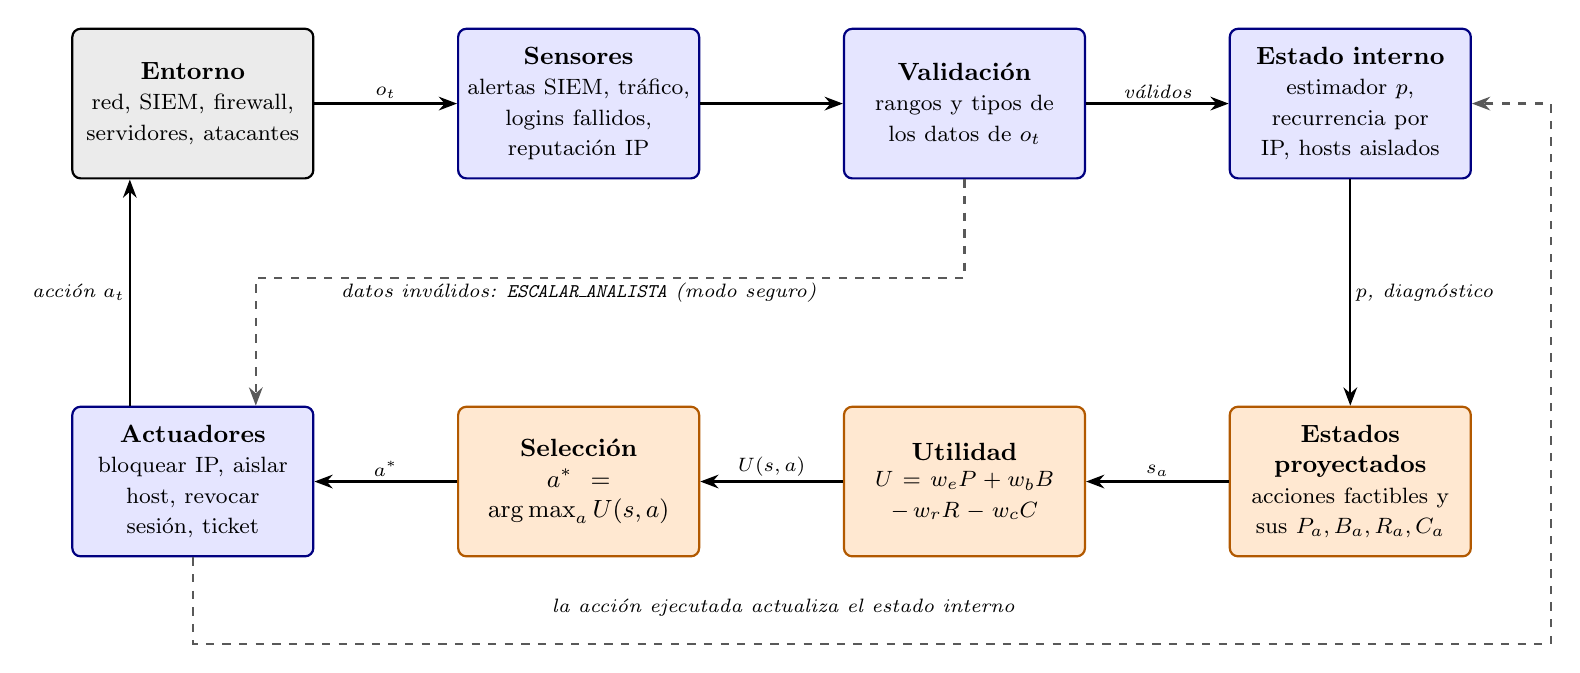
\begin{tikzpicture}[
  font=\small,
  >=Stealth,
  caja/.style={draw, rounded corners=3pt, minimum width=3.0cm, minimum height=1.9cm, align=center, text width=2.85cm, thick, inner sep=3pt},
  ent/.style={caja, fill=black!8},
  ag/.style={caja, fill=blue!10, draw=blue!50!black},
  nucleo/.style={caja, fill=orange!18, draw=orange!70!black},
  flujo/.style={->, thick},
  aux/.style={->, thick, dashed, black!65},
  et/.style={font=\scriptsize\itshape, fill=white, inner sep=1.5pt}
]
% Fila superior (percepción)
\node[ent]  (env)  at (0,0)    {\textbf{Entorno}\\ \footnotesize red, SIEM, firewall, servidores, atacantes};
\node[ag]   (sens) at (4.9,0)  {\textbf{Sensores}\\ \footnotesize alertas SIEM, tráfico, logins fallidos, reputación IP};
\node[ag]   (val)  at (9.8,0)  {\textbf{Validación}\\ \footnotesize rangos y tipos de los datos de $o_t$};
\node[ag]   (est)  at (14.7,0) {\textbf{Estado interno}\\ \footnotesize estimador $p$, recurrencia por IP, hosts aislados};
% Fila inferior (decisión y acción)
\node[ag]     (act)  at (0,-4.8)    {\textbf{Actuadores}\\ \footnotesize bloquear IP, aislar host, revocar sesión, ticket};
\node[nucleo] (sel)  at (4.9,-4.8)  {\textbf{Selección}\\ $a^*=\operatorname{arg\,max}_a U(s,a)$};
\node[nucleo] (util) at (9.8,-4.8)  {\textbf{Utilidad}\\ \footnotesize $U=w_eP+w_bB$\\ $-\,w_rR-w_cC$};
\node[nucleo] (gen)  at (14.7,-4.8) {\textbf{Estados proyectados}\\ \footnotesize acciones factibles y sus $P_a,B_a,R_a,C_a$};

\draw[flujo] (env) -- node[et,above]{$o_t$} (sens);
\draw[flujo] (sens) -- (val);
\draw[flujo] (val) -- node[et,above]{válidos} (est);
\draw[flujo] (est) -- node[et,right]{$p$, diagnóstico} (gen);
\draw[flujo] (gen) -- node[et,above]{$s_a$} (util);
\draw[flujo] (util) -- node[et,above]{$U(s,a)$} (sel);
\draw[flujo] (sel) -- node[et,above]{$a^*$} (act);
\draw[flujo] ($(act.north)+(-0.8,0)$) -- node[et,left]{acción $a_t$} ($(env.south)+(-0.8,0)$);
% Modo seguro: validación -> actuadores
\draw[aux] (val.south) -- ++(0,-1.25) -| ($(act.north)+(0.8,0)$);
\node[et] at (4.9,-2.4) {datos inválidos: \texttt{ESCALAR\_ANALISTA} (modo seguro)};
% Actualización del estado interno
\draw[aux] (act.south) -- ++(0,-1.1) -| ($(est.east)+(1.0,0)$) -- (est.east);
\node[et] at (7.5,-6.4) {la acción ejecutada actualiza el estado interno};
\end{tikzpicture}}
\caption{Arquitectura del agente basado en utilidad para el SOC. El nodo naranja es el núcleo de decisión.}\label{fig:arq}
\end{figure}

El ciclo completo, en cinco pasos que coinciden con los métodos de la implementación (sección~\ref{sec:impl}), es:
\begin{enumerate}
\item \textbf{Percepción y modelo del mundo.} Se validan los sensores y se estima $p$, la probabilidad de que la alerta sea una amenaza real, usando también la memoria del agente (alertas previas de la misma IP, hosts ya aislados). El estado interno se etiqueta como falso positivo probable, incidente ambiguo, amenaza probable, amenaza confirmada o ya contenido.
\item \textbf{Modelo de transición.} Para cada acción factible se proyectan sus consecuencias esperadas en cuatro dimensiones: éxito $P_a$, rapidez $B_a$, riesgo $R_a$ y costo $C_a$.
\item \textbf{Función de utilidad.} Se calcula $U(s,a)$ para cada acción.
\item \textbf{Maximización.} Se elige $a^*=\arg\max_a U(s,a)$.
\item \textbf{Actuación.} Se ejecuta la acción y se actualiza el estado interno y la bitácora.
\end{enumerate}

%====================================================================== 4
\section{Función de utilidad}\label{sec:util}

\subsection{Estimador de amenaza real}

El agente necesita convertir los sensores en una probabilidad $p=\Pr(\text{amenaza real}\mid o_t)$. Se usa un modelo logístico con coeficientes asignados manualmente a partir de criterio experto (no ajustados con datos reales, ver limitaciones):
\begin{equation}
z=\beta_0+\beta_r\,r+\beta_s\,s+\beta_\tau\,\tau+\beta_n\,\frac{\min(n,20)}{20}+\beta_k\,\frac{\min(k,5)}{5}+b_{\text{tipo}},\qquad
p=\frac{1}{1+e^{-z}}.
\end{equation}
Aquí $r$ es la reputación de la IP, $s$ la severidad del SIEM normalizada, $\tau$ el puntaje de tráfico anómalo, $n$ los intentos fallidos de autenticación, $k$ el número de alertas previas de la misma IP y $b_{\text{tipo}}$ un bono para tipos de alerta intrínsecamente graves. Los valores están en la tabla~\ref{tab:coef}. Una combinación logística es razonable porque cada indicio suma evidencia de forma suave y acotada y porque $p$ siempre queda en $(0,1)$.

\begin{table}[H]
\centering
\caption{Coeficientes del estimador de amenaza.}\label{tab:coef}
\small
\begin{tabular}{lcl}
\toprule
Término & Coeficiente & Variable normalizada \\
\midrule
Sesgo $\beta_0$ & $-$3,0 & --- \\
Reputación de la IP & 2,5 & $r\in[0,1]$ \\
Severidad del SIEM & 2,0 & $s=\text{severidad}/10$ \\
Tráfico anómalo & 1,5 & $\tau\in[0,1]$ \\
Intentos fallidos & 2,0 & $\min(n,20)/20$ \\
Recurrencia (estado interno) & 1,5 & $\min(k,5)/5$ \\
Bono por tipo: malware / exfiltración & 1,5 & $b_{\text{tipo}}$ \\
\bottomrule
\end{tabular}

\end{table}

\subsection{Catálogo de acciones}

Cada acción $a$ se describe con cinco parámetros (tabla~\ref{tab:acciones}): su efectividad $e_a$ para contener una amenaza real, el tiempo $t_a$ que tarda en surtir efecto, la interrupción $\kappa_a$ que causa si la alerta era un falso positivo, la probabilidad $f_a$ de que el desenlace sea correcto cuando la alerta era benigna, y su costo operativo $C_a$ (carga humana, tickets, restauración). Aislar contiene casi siempre y casi al instante, pero es la acción más disruptiva ($\kappa=1$); escalar interrumpe poco pero tarda 30 minutos y consume al analista ($C=0{,}80$).

\begin{table}[H]
\centering
\caption{Parámetros del catálogo de acciones.}\label{tab:acciones}
\small
\begin{tabular}{lccccc}
\toprule
Acción $a$ & $e_a$ & $t_a$ (min) & $\kappa_a$ & $f_a$ & $C_a$ \\
\midrule
\texttt{IGNORAR} & 0,00 & 0 & 0,00 & 1,0 & 0,00 \\
\texttt{BLOQUEAR\_IP} & 0,80 & 1 & 0,15 & 0,0 & 0,10 \\
\texttt{REVOCAR\_CREDENCIALES} & 0,70 & 2 & 0,35 & 0,0 & 0,15 \\
\texttt{AISLAR\_HOST} & 0,95 & 1 & 1,00 & 0,0 & 0,30 \\
\texttt{ESCALAR\_ANALISTA} & 0,90 & 30 & 0,05 & 1,0 & 0,80 \\
\bottomrule
\end{tabular}

\end{table}

\subsection{Componentes de la utilidad}

Sean $p$ la probabilidad de amenaza real, $s\in[0,1]$ la severidad normalizada del SIEM y $c\in[0,1]$ la criticidad del activo afectado. Con $T_{\max}=60$ min, la ventana máxima de contención, se define la rapidez $\rho_a=1-t_a/T_{\max}$ y los cuatro componentes de un estado proyectado:
\begin{align}
P_a &= p\,e_a+(1-p)\,f_a, \\
B_a &= 100\,\rho_a, \\
R_a &= \underbrace{(1-p)\,\kappa_a\,c}_{\text{interrupción por falso positivo}}+\underbrace{p\,s\,\bigl(1-e_a\rho_a\bigr)}_{\text{amenaza residual}}, \\
C_a &= \text{costo operativo de la tabla~\ref{tab:acciones}.}
\end{align}
Aquí $P_a$ es la probabilidad de un desenlace correcto, $B_a$ el beneficio operativo (rapidez con que se cierra el incidente), $R_a$ el riesgo de impacto y $C_a$ el costo de intervención.
El riesgo $R_a$ penaliza los dos errores posibles con la misma moneda. El primer término es el costo de \emph{actuar de más}: crece con la probabilidad de que la alerta sea benigna, con la disrupción de la acción y con la criticidad del activo. El segundo es el costo de \emph{actuar de menos}: crece con la probabilidad de amenaza real, con su severidad y con la fracción que la acción no logra contener a tiempo. Ignorar tiene $e=0$, así que su riesgo es $p\,s$, y escalar deja una amenaza residual porque la contención demora 30 minutos.

\subsection{Función de utilidad y política óptima}

La utilidad de ejecutar la acción $a$ en el estado $s$ es
\begin{equation}
U(s,a)=w_e\,P_a+w_b\,B_a-w_r\,R_a-w_c\,C_a,
\qquad a^*=\argmax_{a\in\mathcal{F}(s)}U(s,a),
\end{equation}
donde $\mathcal{F}(s)$ es el conjunto de acciones factibles. Los pesos usados son
\[
w_e=100,\qquad w_b=0{,}5,\qquad w_r=400,\qquad w_c=30.
\]
Su justificación es la siguiente. Como $P_a\in[0,1]$ y $B_a\in[0,100]$, el producto $w_eP_a$ aporta hasta 100 puntos y $w_bB_a$ hasta 50, de manera que la rapidez cuenta pero nunca domina sobre el éxito. La penalización al riesgo es la más fuerte ($w_r=400$, cuatro veces $w_e$), porque en seguridad un error costoso (aislar un servidor crítico sano, o dejar pasar un ataque severo) pesa más que cualquier ganancia de velocidad. El costo operativo con $w_c=30$ desempata entre acciones parecidas, favoreciendo las que no consumen al analista. Estos valores se fijaron por razonamiento sobre las escalas y se verificaron con los escenarios y con el análisis de sensibilidad de la sección~\ref{sec:pruebas}.

\subsection{Ejemplo numérico}

Se toma el evento EVT-06: malware en un servidor crítico, con $p=\ejP$, $s=\ejS$ y $c=\ejC$. Para aislar el host ($e=0{,}95$, $t=1$ min, $\kappa=1$, $\rho=0{,}983$):
\begin{align*}
P&=0{,}979\cdot0{,}95+0{,}021\cdot0=0{,}930, & B&=100\cdot0{,}983=98{,}3,\\
R&=0{,}021\cdot1\cdot0{,}95+0{,}979\cdot0{,}95\,(1-0{,}95\cdot0{,}983)=0{,}081, & C&=0{,}30,
\end{align*}
\[
U=100(0{,}930)+0{,}5(98{,}3)-400(0{,}081)-30(0{,}30)\approx 100{,}8.
\]
La tabla~\ref{tab:ejemplo} compara las cuatro acciones factibles. Escalar al analista tiene un riesgo alto ($R=0{,}513$) porque la amenaza casi segura tendría 30 minutos para propagarse, e ignorar es catastrófico. Aislar gana aunque sea la acción más disruptiva, porque la probabilidad de que el servidor esté sano es de solo 2\,\%.

\begin{table}[H]
\centering
\caption{Utilidad de cada acción factible en el evento EVT-06.}\label{tab:ejemplo}
\small
\begin{tabular}{lrrrrr}
\toprule
Acción $a$ & $P_a$ & $B_a$ & $R_a$ & $C_a$ & $U(s,a)$ \\
\midrule
\texttt{AISLAR\_HOST} & 0,930 & 98,3 & 0,081 & 0,30 & 100,77 \\
\texttt{BLOQUEAR\_IP} & 0,783 & 98,3 & 0,201 & 0,10 & 43,93 \\
\texttt{ESCALAR\_ANALISTA} & 0,902 & 50,0 & 0,513 & 0,80 & $-$113,83 \\
\texttt{IGNORAR} & 0,021 & 100,0 & 0,930 & 0,00 & $-$320,00 \\
\bottomrule
\end{tabular}

\end{table}

%====================================================================== 5
\section{Implementación en Python}\label{sec:impl}

El prototipo se escribió en Python usando solo la biblioteca estándar, a partir de la plantilla del taller (clases \texttt{Percepcion}, \texttt{EstadoProyectado} y \texttt{AgenteBasadoEnUtilidad}). La separación de responsabilidades es la siguiente:
\begin{itemize}
\item \texttt{modelos.py}: estructuras de datos y validación de los sensores (\texttt{Percepcion.validar}).
\item \texttt{base.py}: clase abstracta con el ciclo genérico de un agente basado en utilidad; define \texttt{calcular\_utilidad} y \texttt{seleccionar\_mejor\_accion}.
\item \texttt{config.py}: todos los parámetros (pesos, catálogo de acciones, coeficientes) en un único lugar, para recalibrar sin tocar la lógica.
\item \texttt{agente\_soc.py}: la clase concreta \texttt{AgenteSOC} con el estimador de amenaza, las acciones factibles, los estados proyectados y los actuadores simulados.
\item \texttt{escenarios.py} y \texttt{simulacion.py}: casos de prueba nombrados y simulación con verdad de terreno para medir los KPIs.
\end{itemize}

Los cinco pasos del ciclo de la figura~\ref{fig:arq} se corresponden uno a uno con métodos: \texttt{actualizar\_estado\_interno} (paso 1), \texttt{generar\_estados\_proyectados} y \texttt{proyectar} (paso 2), \texttt{calcular\_utilidad} (paso 3), \texttt{seleccionar\_mejor\_accion} (paso 4) y \texttt{ejecutar\_actuador} (paso 5). El listado~\ref{lst:util} muestra el núcleo matemático y el listado~\ref{lst:proy} la proyección de cada acción, que implementa literalmente las ecuaciones de la sección~\ref{sec:util}.

\lstinputlisting[caption={Función de utilidad $U(s,a)$ (\texttt{base.py}).},label={lst:util}]{generado/cod_utilidad.py}

\lstinputlisting[caption={Proyección de una acción: $P_a$, $B_a$, $R_a$ y $C_a$ (\texttt{agente\_soc.py}).},label={lst:proy}]{generado/cod_proyectar.py}

\lstinputlisting[caption={Maximización de la utilidad (\texttt{base.py}).},label={lst:sel}]{generado/cod_seleccion.py}

\paragraph{Tolerancia a fallos.} El agente sigue el principio de diseñar para el fallo. \texttt{Percepcion.validar} lanza \texttt{ValueError} ante sensores ausentes, tipos desconocidos o valores fuera de rango, y \texttt{procesar\_evento\_seguro} captura esas excepciones y responde escalando al analista con un ticket de prioridad alta, en lugar de decidir con datos corruptos o dejar caer el proceso (listado~\ref{lst:seguro}).

\lstinputlisting[caption={Modo seguro ante datos inválidos (\texttt{agente\_soc.py}).},label={lst:seguro}]{generado/cod_seguro.py}

\paragraph{Estado interno.} El agente recuerda cuántas alertas ha visto por IP (alimenta el término de recurrencia $k$), qué hosts están aislados, qué IP están bloqueadas y qué tickets abrió. Si llega una alerta sobre un host ya aislado, el diagnóstico es \texttt{YA\_CONTENIDO} y la única acción es ignorar: no tiene sentido volver a aislar ni escalar algo ya contenido.

%====================================================================== 6
\section{Casos de prueba y métricas de evaluación}\label{sec:pruebas}

\subsection{Escenarios}

Se definieron nueve escenarios: dos rutinarios, tres ambiguos, dos críticos y dos extremos. Todos se ejecutan con \texttt{python main.py} y se verifican de forma automática en las pruebas unitarias. La tabla~\ref{tab:escenarios} resume la decisión del agente.

\begin{table}[H]
\centering
\caption{Resultados de los escenarios de prueba. $p$ es la probabilidad de amenaza estimada y $U^*$ la utilidad de la acción elegida.}\label{tab:escenarios}
\scriptsize
\begin{tabularx}{\textwidth}{llXcccc}
\toprule
ID & Categoría & Descripción & $p$ & Decisión del agente & $U^*$ & OK \\
\midrule
EVT-01 & Rutinario & Escaneo de puertos de baja severidad desde IP con buena reputación & 0,14 & \texttt{IGNORAR} & 120,11 & \checkmark \\
EVT-02 & Rutinario & Un único fallo de login en estación, origen interno & 0,09 & \texttt{IGNORAR} & 133,60 & \checkmark \\
EVT-03 & Ambiguo & Usuario legítimo (posible olvido de clave): 10 fallos, IP de reputación baja & 0,41 & \texttt{ESCALAR\_ANALISTA} & 47,87 & \checkmark \\
EVT-04 & Ambiguo & Inicio de sesión anómalo en servidor crítico, origen interno, evidencia mixta & 0,57 & \texttt{ESCALAR\_ANALISTA} & 11,34 & \checkmark \\
EVT-05 & Ambiguo & Posible exfiltración desde servidor crítico hacia IP externa (contención de menor impacto) & 0,79 & \texttt{BLOQUEAR\_IP} & 56,59 & \checkmark \\
EVT-06 & Crítico & Malware confirmado en servidor crítico, IP maliciosa conocida & 0,98 & \texttt{AISLAR\_HOST} & 100,77 & \checkmark \\
EVT-07 & Crítico & Fuerza bruta masiva desde IP maliciosa contra una estación & 0,93 & \texttt{AISLAR\_HOST} & 103,76 & \checkmark \\
EVT-08 & Extremo & Sensor corrupto: severidad fuera de rango (fail-safe) & --- & \texttt{ESCALAR\_ANALISTA} & --- & \checkmark \\
EVT-09 & Extremo & Todos los indicadores al máximo en servidor crítico & 1,00 & \texttt{AISLAR\_HOST} & 108,13 & \checkmark \\
\bottomrule
\end{tabularx}

\end{table}

Los resultados muestran el comportamiento buscado. En los casos rutinarios, donde $p$ es baja, el agente ignora sin consumir recursos. En los ambiguos escala al analista, y en el caso EVT-05, donde la evidencia es mixta pero el origen es externo y el activo es crítico, prefiere la acción de menor impacto que aún contiene (bloquear la IP) frente a aislar el servidor. En los críticos aísla el host. En el caso EVT-08, con un sensor corrupto, no intenta decidir y escala (modo seguro).

Dos comportamientos dinámicos adicionales se verifican en las pruebas unitarias: una alerta que se ignoraría por sí sola deja de ignorarse cuando se repite desde la misma IP (la recurrencia eleva $p$), y una alerta sobre un host ya aislado se ignora.

\subsection{Pruebas unitarias}

El archivo \texttt{tests/test\_agente.py} contiene 16 pruebas que se ejecutan con \texttt{pytest} o con \texttt{unittest}. Cubren: la coincidencia de cada escenario con su acción esperada; la forma de la función de utilidad (cálculo exacto, rango de $p$, monotonía respecto a la reputación); el efecto de los parámetros (un servidor crítico desplaza la decisión hacia acciones menos disruptivas, y con $w_r=0$ el agente ignora casos ambiguos, lo que confirma el papel del peso de riesgo); el estado interno (host ya aislado, recurrencia, factibilidad de bloquear solo IP externas); la validación y el modo seguro; y la reproducibilidad y calidad de la simulación.

\subsection{Simulación con verdad de terreno}

Para medir los KPIs se generaron 1000 alertas sintéticas con una semilla fija, de las cuales el 15\,\% son amenazas reales (\nAmenazas{} en la muestra). Los sensores se muestrean según la etiqueta real (por ejemplo, las amenazas tienen mayor reputación de IP y severidad), y el tipo de activo se reparte en 60\,\% estaciones, 25\,\% servidores internos y 15\,\% servidores críticos. Cada política se aplica sobre los mismos eventos y los mismos números aleatorios, de modo que la comparación es justa. El resultado de una acción se simula con las probabilidades del catálogo: una amenaza se contiene con probabilidad $e_a$ y una alerta benigna sufre interrupción con probabilidad $\kappa_a$. Se compara con dos líneas base: \emph{reglas if-else} (aislar si la severidad del SIEM es al menos 7, ignorar en otro caso) y \emph{siempre escalar}.

\begin{table}[H]
\centering
\caption{KPIs sobre 1000 alertas simuladas (semilla 42). FP = falsos positivos con acción disruptiva efectiva.}\label{tab:kpis}
\scriptsize
\begin{tabular}{lrrrrrr}
\toprule
Política & MTTC (min) & Bloqueo efectivo & No contenidas & Interrup. críticas & FP afectados & Escalamiento \\
\midrule
Agente (utilidad) & 1,23 & 94,7\,\% & 7 & 1 & 49 & 17,0\,\% \\
Reglas if-else & 1,00 & 51,1\,\% & 65 & 0 & 15 & 0,0\,\% \\
Siempre escalar & 30,00 & 89,5\,\% & 14 & 0 & 0 & 100,0\,\% \\
\bottomrule
\end{tabular}

\end{table}

La tabla~\ref{tab:kpis} permite tres lecturas. Primero, el agente contiene la gran mayoría de las amenazas reales con un MTTC de poco más de un minuto, frente a 30 minutos de escalar todo, y con una tasa de bloqueo muy superior a la de las reglas rígidas, que dejan sin contener casi la mitad de las amenazas (las que tienen severidad moderada pero otros indicios claros). Segundo, escalar todo logra cero interrupciones, pero a costa de saturar al analista (100\,\% de las alertas) y de una contención 24 veces más lenta; el agente solo escala la parte ambigua (alrededor del 17\,\%). Tercero, la meta de cero interrupciones a servicios críticos \emph{no se cumple del todo}: hay una interrupción, producida por una acción de contención de baja disrupción sobre un servidor crítico. Es una consecuencia directa del compromiso modelado y no un defecto del código, y para reducirla a cero habría que aceptar más escalamientos, lo que muestra el análisis de sensibilidad.

\subsection{Sensibilidad al peso de riesgo}

El parámetro con más influencia en el dilema es $w_r$. La figura~\ref{fig:sens} y la tabla~\ref{tab:sens} muestran qué ocurre al variarlo entre 50 y 1600 manteniendo el resto fijo.

\begin{figure}[H]
\centering
\begin{tikzpicture}
\begin{axis}[
  width=0.85\textwidth, height=6.2cm, xmode=log, log basis x=2,
  xlabel={Peso de riesgo $w_r$}, ylabel={\%}, ymin=0, ymax=105,
  xtick={50,100,200,400,800,1600}, xticklabels={50,100,200,400,800,1600},
  legend style={font=\footnotesize, at={(0.97,0.68)}, anchor=north east}, grid=major, grid style={black!15}]
\addplot[blue!70!black, mark=*, thick] table[x index=0, y index=1] {generado/sens_bloqueo.dat};
\addlegendentry{Bloqueo efectivo de amenazas}
\addplot[orange!80!black, mark=square*, thick] table[x index=0, y index=1] {generado/sens_escalamiento.dat};
\addlegendentry{Alertas escaladas a un analista}
\draw[dashed, black!60] (axis cs:400,0) -- (axis cs:400,105);
\end{axis}
\end{tikzpicture}
\caption{Efecto del peso de riesgo $w_r$ sobre la tasa de bloqueo y la carga del analista (la línea discontinua marca el valor adoptado, $w_r=400$).}\label{fig:sens}
\end{figure}

\begin{table}[H]
\centering
\caption{Sensibilidad de los KPIs al peso de riesgo $w_r$.}\label{tab:sens}
\small
\begin{tabular}{rrrrr}
\toprule
$w_r$ & Bloqueo efectivo & No contenidas & FP afectados & Escalamiento \\
\midrule
50 & 96,2\,\% & 5 & 59 & 4,3\,\% \\
100 & 95,5\,\% & 6 & 54 & 6,8\,\% \\
200 & 94,7\,\% & 7 & 49 & 10,3\,\% \\
400 & 94,7\,\% & 7 & 49 & 17,0\,\% \\
800 & 94,0\,\% & 8 & 51 & 27,0\,\% \\
1600 & 94,0\,\% & 8 & 59 & 33,8\,\% \\
\bottomrule
\end{tabular}

\end{table}

A medida que $w_r$ crece, el agente escala cada vez más alertas (de 4\,\% a 34\,\%), porque escalar es la acción de menor disrupción. La tasa de bloqueo baja levemente y los falsos positivos afectados no disminuyen de forma monótona: con $w_r$ muy alto el término de amenaza residual de ignorar también pesa más, y el agente reemplaza parte de los ``ignorar'' por \texttt{BLOQUEAR\_IP}, una acción de bajo impacto, sobre alertas de probabilidad intermedia (en la simulación, los bloqueos sobre eventos benignos pasan de 42 con $w_r=400$ a 97 con $w_r=1600$). El valor $w_r=400$ queda en una zona estable: entre 200 y 400 la tasa de bloqueo y los falsos positivos casi no cambian, y la carga del analista se mantiene razonable.

\subsection{Limitaciones}

Las cifras corresponden a datos sintéticos y a un modelo de resultados simplificado, así que sirven para comparar políticas entre sí, no para predecir el desempeño en una red real. Los parámetros $e_a$, $t_a$, $\kappa_a$ y los coeficientes del estimador se asignaron por criterio y no se ajustaron con alertas históricas de un SIEM. Además, el prototipo no se conecta a un SIEM ni a un firewall reales: los actuadores son simulados y registran su efecto en una bitácora.

%====================================================================== 7
\section{Conclusiones y trabajo futuro}\label{sec:conclusiones}

Se diseñó e implementó un agente de triaje para un SOC cuyo comportamiento sale de una función de utilidad explícita y no de reglas fijas. El modelo PEAS y la clasificación del entorno justifican la arquitectura: como el entorno es parcialmente observable, estocástico y dinámico, el agente mantiene un estado interno, razona con probabilidades y tiene en cuenta el tiempo de reacción. La función $U(s,a)$ expresa el dilema del proyecto, porque la rapidez entra como beneficio y el costo de desconectar por error como parte del riesgo, ponderado por la criticidad del activo.

En la simulación, el agente contuvo el 94{,}7\,\% de las amenazas reales con un MTTC de 1{,}23 minutos, frente al 51{,}1\,\% de las reglas rígidas y a los 30 minutos de escalar todo, escalando solo el 17\,\% de las alertas. La meta de cero interrupciones a servicios críticos no se alcanzó (hubo una), y el análisis de sensibilidad muestra que reducirla implica escalar más.

Como trabajo futuro se proponen tres líneas: calibrar los coeficientes y parámetros con alertas reales y la retroalimentación de los analistas (la parte de aprendizaje de un diseño híbrido completo); desplegar primero en modo sombra, donde el agente recomienda pero no actúa, y luego de forma gradual (\emph{canary}), como recomienda el taller; y conectar los sensores y actuadores a un SIEM y un firewall reales.

\begin{thebibliography}{9}
\bibitem{aima} Russell, S. y Norvig, P. (2021). \emph{Artificial Intelligence: A Modern Approach} (4.ª ed.). Pearson.
\bibitem{taller} Taller de Ingeniería de Agentes Inteligentes: de los fundamentos a los sistemas multi-agente (noviembre de 2026). Material del curso, Fundación Universitaria Los Libertadores.
\end{thebibliography}

%====================================================================== Anexo
\appendix
\section{Repositorio y ejecución}\label{sec:repo}

\begin{lstlisting}[language=bash,numbers=none,caption={Estructura del repositorio.}]
soc-agent/
  main.py                  # ejecuta escenarios + simulacion + KPIs
  requirements.txt
  soc_agent/
    modelos.py             # Percepcion (sensores) y EstadoProyectado
    base.py                # AgenteBasadoEnUtilidad (ciclo generico)
    config.py              # pesos, catalogo de acciones, coeficientes
    agente_soc.py          # AgenteSOC (estimador, factibilidad, actuadores)
    escenarios.py          # 9 casos de prueba nombrados
    simulacion.py          # simulacion con verdad de terreno y KPIs
  tests/test_agente.py     # 16 pruebas unitarias
  resultados/              # salidas de main.py (json, csv, consola)
  docs/                    # informe.tex, informe.pdf, generar_tablas.py
\end{lstlisting}

\begin{lstlisting}[language=bash,numbers=none,caption={Ejecución.}]
python main.py                   # escenarios y simulacion
python -m pytest -q              # pruebas (o: python -m unittest discover tests)
python docs/generar_tablas.py    # regenera las tablas del informe desde el codigo
cd docs && pdflatex informe.tex && pdflatex informe.tex
\end{lstlisting}

\end{document}
